\subsection{Verwandte Arbeiten}
\begin{frame}
  \frametitle{\currentsectionname}

  % \note{
  %   \begin{itemize}
  %   \end{itemize}
  % }

\end{frame}

\begin{frame}
  \frametitle{DataSnap}

  \begin{minipage}{.6\textwidth}
    \begin{itemize}
      \item Weiterentwicklung von \textit{Snap!}, die an Fachexpert:innen gerichtet ist.
      \item Einfaches Importieren von Daten.
      \item Nutzung von externen Rechnern zur Beschleunigung der Auswertung.
      \item Benutzung von \textit{Snap!}-Blöcken zur Definition der Datenverarbeitung.
    \end{itemize}
  \end{minipage}%
  \begin{minipage}{.4\textwidth}
    \begin{figure}
      \begin{center}
        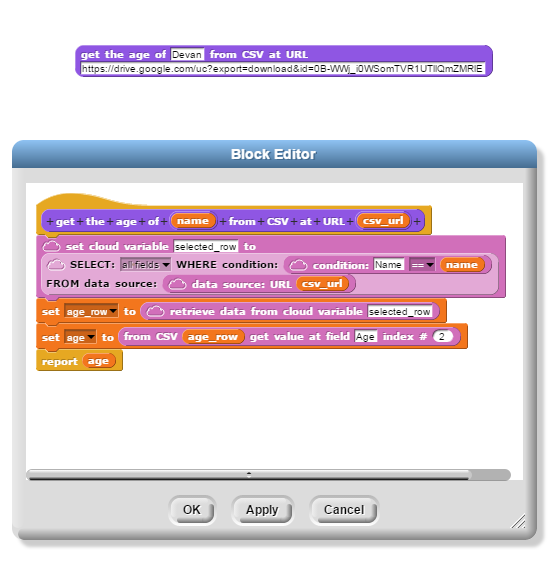
\includegraphics[width=0.95\textwidth]{assets/datasnap-block-definition.png}
      \end{center}
      \caption{Definition eines Blocks in \textit{DataSnap}. \parencite[26]{hellmannDataSnapEnabling2015}}
    \end{figure}
  \end{minipage}

  \Note{
    \item Masterarbeit
    \item Importieren über diesen dunkelpinken Block "data source"
    \item Abspeichern in sog. cloud variablen - auf externem Rechner, also Server
    \item auf dem Server können dann auch Berechnungen ausgeführt werden, weniger abhängig vom Client
    \item Hier rechts wird die Funktionalität als Block definiert, um später in anderen Abfragen schnell wiederverwendet zu werden
  }

\end{frame}

\begin{frame}
  \frametitle{DataSnap (cont.)}

  \begin{itemize}
    \item Visualisierung der Ergebnisse.
  \end{itemize}
  \begin{figure}
    \begin{center}
      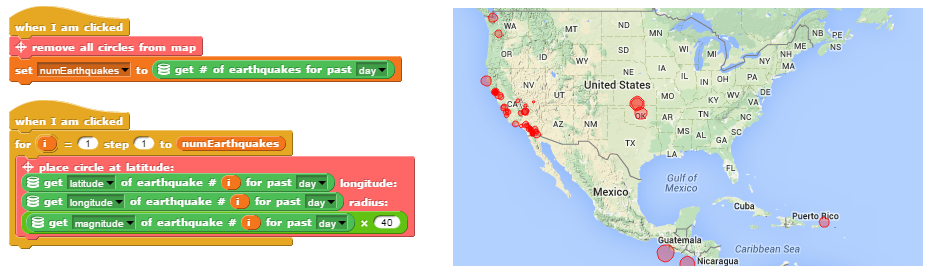
\includegraphics[width=0.95\textwidth]{assets/datasnap-visualization.png}
    \end{center}
    \caption{Visualisierung von Erdbeben mit \textit{DataSnap}. \parencite[28]{hellmannDataSnapEnabling2015}}
  \end{figure}

  \Note{
    \item mithilfe von standard Snap! und neu eingeführten Blöcken Visualisierung möglich
    \item Hier z.B. Erdbeben in Nordamerika mit Darstellung der Magnitude in Form des Radius der Kreise
  }

\end{frame}
